\section{Microservice Architecture}

The microservice architectural style is an approach to developing a single application as a suite of small services, each running in its own process and communicating with lightweight mechanisms, often \hl{an HTTP resource API}. These services are built around business capabilities and independently deployable by fully automated deployment machinery. \hl{There is a bare minimum of centralized management of these services, which may be written in different programming languages and use different data storage technologies} \cite{LewisMicroservices}.

\hl{Among the characteristics of microservice, a few characteristics heavily affect while moving from} \acrshort{soa} to microservice.
\dbc{M in Microservice should be capitalized only on begining of a sentence.}

%%%%%%%%%%%%%%%%%%%%%%%%%%%%%%%%%%%%%%%%%%%%%%%%%%%%%%%%%%%%%%%%%%%%%%%%%%%%%%%%
\subsection{Smart Endpoints and Dumb Pipes}
\label{subse:dumb_pipes}
\dbc{At the end of previous para tell what will be discussed in the next set of sub-section. A single sentence like "Next, we will discusss ...." is enough}

When building communication endpoints, \hl{many architecture approach with putting significant smart into the communication mechanism.} One good example is \acrshort{esb} what we discussed in Section \ref{se:architectural_decisions}. But microservice follows alternative approach: \emph{Smart endpoints and dumb pipes} \cite{LewisMicroservicesPipes}.
Applications built from microservices aim to be as decoupled and as cohesive as possible. They own their own domain logic and act more as filters in the classical Unix sense. After receiving a request, applying logic as appropriate and producing a response. And it uses simple RESTish protocols rather than complex protocols.
\dbc{RESTish or RESTful?}

%%%%%%%%%%%%%%%%%%%%%%%%%%%%%%%%%%%%%%%%%%%%%%%%%%%%%%%%%%%%%%%%%%%%%%%%%%%%%%%%
\subsection{\hl{Pattern: Database per Service}}
\label{subse:database_per_service}
\hl{- Pattern: Database per service} 

\acrshort{microservice} prefer letting each service manages its own database, either different instances of the same database technology, or entirely different database systems - an approach called \emph{Polyglot Persistence} \cite{LewisMicroservicesManagement}.

Keep each microservice’s persistent data private to that service and accessible only via its API. 
There are a few different ways to keep a service’s persistent data private. You do not need to provision a database server for each service. For example, if you are using a relational database then the options are \cite{RichardsonMicroservicesService}:
\begin{itemize}
    \item \emph{Private-tables-per-service} –- each service owns a set of tables that must only be accessed by that service
    \item \emph{Schema-per-service} –- each service has a database schema that’s private to that service
    \item \emph{Database-server-per-service} -– each service has its own database server.
\end{itemize}
Private-tables-per-service and schema-per-service have the lowest overhead. Using a schema per service is appealing since it makes ownership clearer. Some high throughput services might need their own database server.

%%%%%%%%%%%%%%%%%%%%%%%%%%%%%%%%%%%%%%%%%%%%%%%%%%%%%%%%%%%%%%%%%%%%%%%%%%%%%%%%
\subsection{\hl{Pattern: Sagas}}
\label{subse:sagas}
In order to ensure loose coupling, each service has its own database. Maintaining data consistency between services is a challenge because 2 phase-commit/distributed transactions is not an option for many applications. An application must instead use the Saga pattern. A service publishes an event when its data changes. Other services consume that event and update their data \cite{RichardsonMicroservicesSagas}.

%%%%%%%%%%%%%%%%%%%%%%%%%%%%%%%%%%%%%%%%%%%%%%%%%%%%%%%%%%%%%%%%%%%%%%%%%%%%%%%%
\subsection{\hl{The Scale Cube}}
\label{subse:scale_cube}
The scalability of a system can explain via a concept called \emph{Scale Cube} which talk about the scalability of the application throw X, Y and Z axis.

\paragraph{x-axis Saling}-- x-axis scaling consists of running multiple copies of an application behind a load balancer. If there are \textit{n} copies then each copy handles 1/\textit{n} of the load. This is a simple, commonly used approach of scaling an application \hl{TODO}.

\paragraph{y-axis Scaling}-- Unlike x-axis and x-axis, which consist of running multiple, identical copies of the application, y-axis axis scaling splits the application into multiple, different services. Each service is responsible for one or more closely related functions. There are a couple of different ways of decomposing the application into services.
\begin{itemize}
    \item verb-based decomposition ex: checkout.
    \item decompose the application by noun, for e.g., customer management. 
    \item An application might use a combination of verb-based and noun-based decomposition.
\end{itemize}
    
The microservice architecture is an application of Y-axis scaling.

\paragraph{Z-axis Scaling}-- When using x-axis scaling each server runs an identical copy of the code (similar to X-axis scaling). The big difference is that each server is responsible for only a subset of the data. 
Z-axis splits are commonly used to scale databases. Data is partitioned (a.k.a. sharded) across a set of servers based on an attribute of each record.

Even \acrshort{wdias} is design based on the Y-axis scaling, it's possible to use the Z-axis scaling to scalability of the system further. This will be more discuss in the Section \ref{se:discussion}.

%%%%%%%%%%%%%%%%%%%%%%%%%%%%%%%%%%%%%%%%%%%%%%%%%%%%%%%%%%%%%%%%%%%%%%%%%%%%%%%%
\subsection{Brief introduction to the \acrfull{k8s}}
\label{sebse:k8s_intro}
\dbc{Don't present this as a separate section. Either this need to be in the literature survey, or integrate key ideas into another section as a paragraph.}

\acrfull{k8s} is an open-source system for automating deployment, scaling, and management of containerized applications \cite{LinuxFoundationProduction-GradeKubernetes}. It groups containers that make up an application into logical units for easy management and discovery.
\begin{figure}[htp]
    \centering
    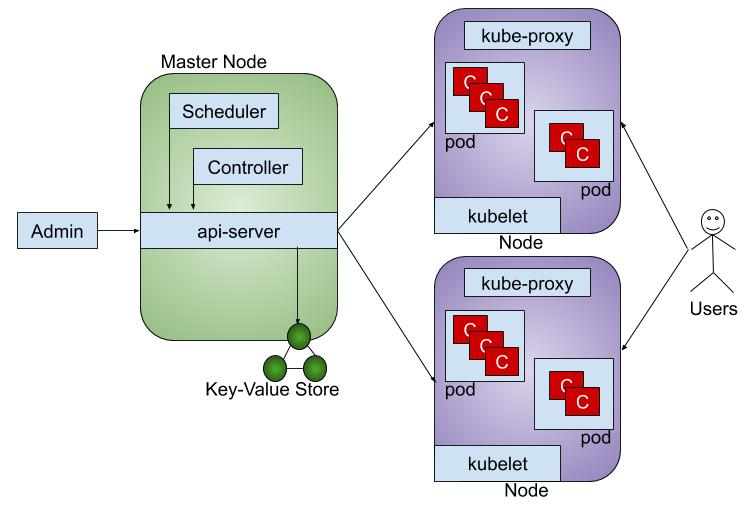
\includegraphics[width=1\textwidth]{method/microservice/k8s_architecture_v3.jpg}
    \caption{\acrfull{k8s} architecture.}
    \label{fi:k8s_architecture}
\end{figure}
Components of \acrshort{k8s},
\begin{itemize}
    \item Pods -- Cluster of containers that can group other container images in a single unit.
    \item Nodes -- the machines (VMs, physical servers, etc) in a cluster that run your applications and cloud workflows.
    \item kubelet -- An agent that runs on each node in the cluster. It makes sure that containers are running in a pod.
    \item kube-proxy -- A network proxy that runs on each node in the cluster, and maintains network rules on nodes.
    \item Kubernetes master -- Responsible for maintaining the desired state for your cluster.
    \item etcd -- Consistent and highly-available key value store used as Kubernetes’ backing store for all cluster data.
\end{itemize}
Users can add much as required Nodes into the \acrshort{k8s} cluster, and \acrshort{k8s} manage and deploy application as pods into cluster nodes.
Each microservice can deploy as a Pod which is a group of containerize applications. And \acrshort{k8s} able to scale as much as user want as described above.


%%%%%%%%%%%%%%%%%%%%%%%%%%%%%%%%%%%%%%%%%%%%%%%%%%%%%%%%%%%%%%%%%%%%%%%%%%%%%%%%
\subsection{\acrshort{wdias} Microservices}
\label{sebse:wdias_microservices}
As seen in Figure of Figure \ref{fi:wdias_micro_on_demand} and Figure \ref{fi:wdias_micro_async} each circle represents a microservice, and those are implemented as containerized applications.
\begin{figure}[htp]
    \centering
    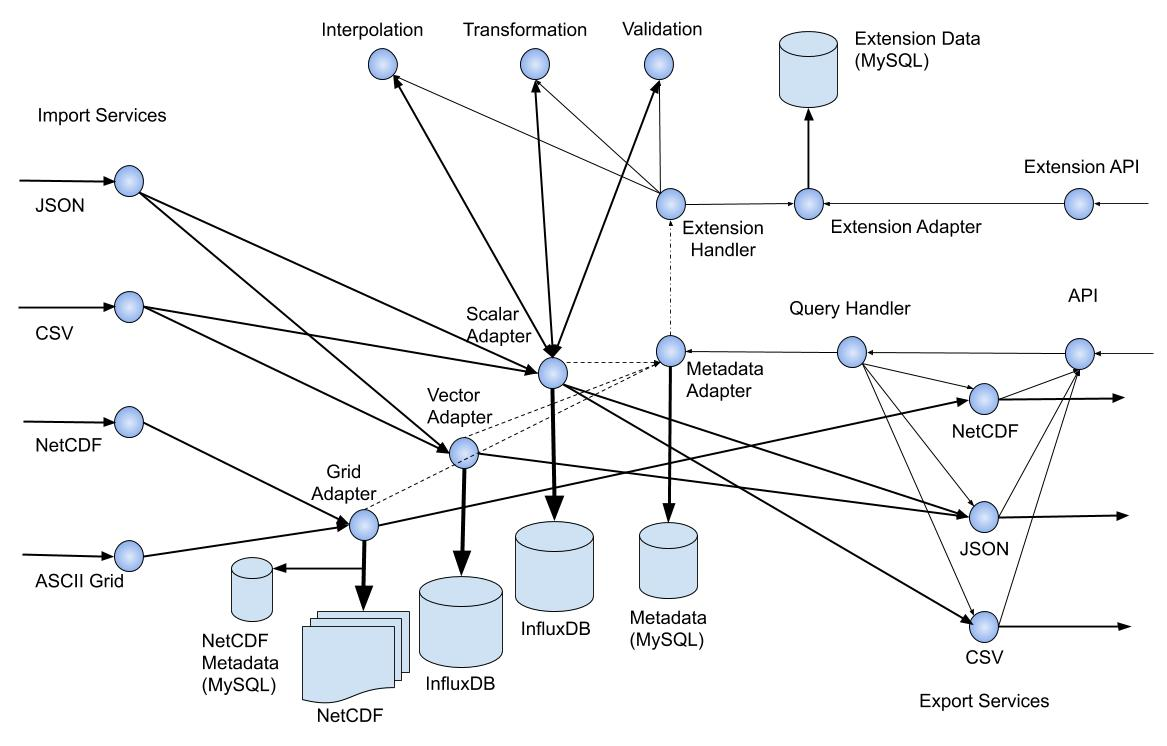
\includegraphics[width=1\textwidth]{method/microservice/microservice_architecture-handle_on_demand-v3.jpg}
    \caption{\acrshort{wdias} architecture \hl{for server requests on demand}}
    \label{fi:wdias_micro_on_demand}
\end{figure}
Left side of Figure \ref{fi:wdias_micro_on_demand} shows the import modules of the \acrshort{wdias}, and right side shows the export modules. As it explained section Section \ref{subse:dumb_pipes}, each import microservice only do specific task of converting and forwarding the request to the correct data adapter module.
For each data type, there is a adapter microservice is running which is optimized to storing such type of data. And the metadata data of the timeseries store using \acrshort{rdbms} which gives more performance over retrieving metadata data. The metadata is cached with In-Memory database to fast access as mentioned in Section \ref{subse:redis}.
The system generate a unique identifier for each timeseries, and throw out the \acrshort{wdias}, other microservice use it to handle data for fast access.

\begin{figure}[htp]
    \centering
    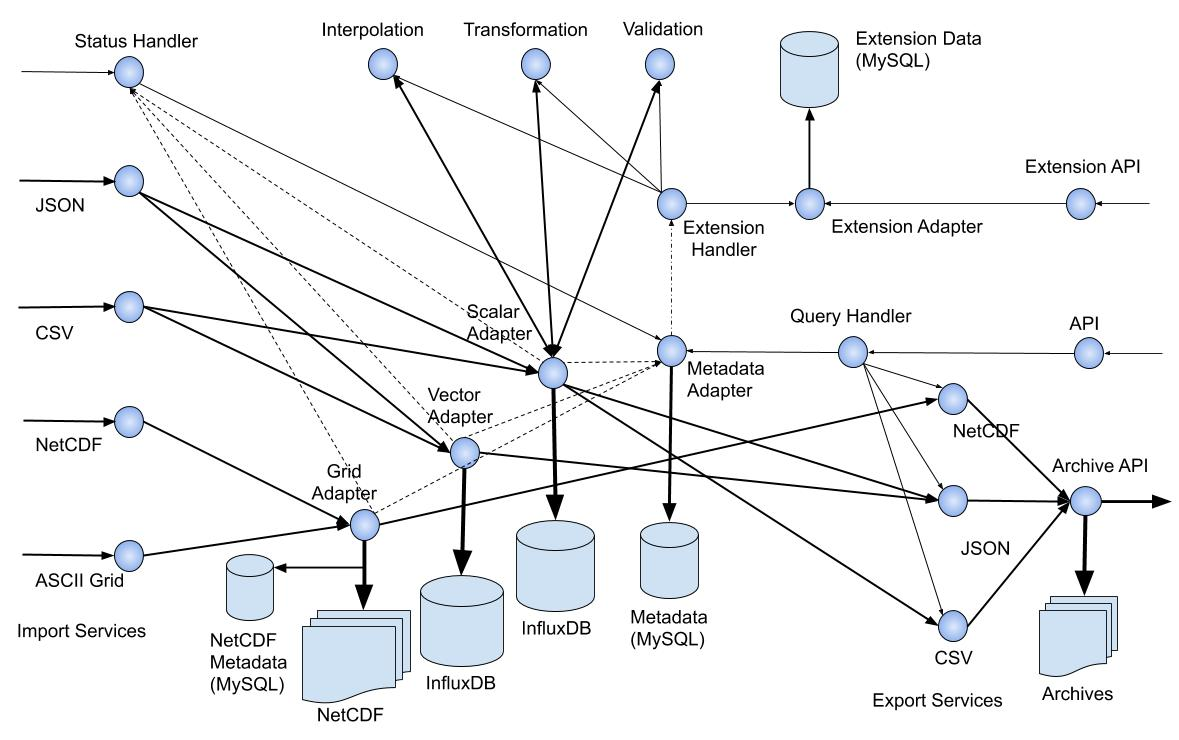
\includegraphics[width=1\textwidth]{method/microservice/microservice_architecture-handle_on_async-v3.jpg}
    \caption{\acrshort{wdias} architecture for handling requests asynchronously.}
    \label{fi:wdias_micro_async}
\end{figure}
Export module microservice follows the same concepts and provide the capability to export the data into required formats of the weather models.
Each adapter follows the concept of database per service as mentioned in the section Section \ref{subse:database_per_service}. This gives the freedom for \acrshort{wdias} to scale better with \acrshort{k8s}.

As shown in Figure \ref{fi:wdias_micro_on_demand}, when a smaller size request come to the system, it handle on demand and response back. However, as shown in Figure \ref{fi:wdias_micro_async}, when a request with larger size come to the system, it store the data for asynchronously process the data and response with a unique id which can use to verify whether data processed successfully or not. Here is uses the microservice pattern of Section \ref{subse:sagas} while processing the Grid data. First it store the data and respond back to the user. Then publish an event, and another service listen to those events and process the data and update the system status.

\begin{figure}[htp]
    \centering
    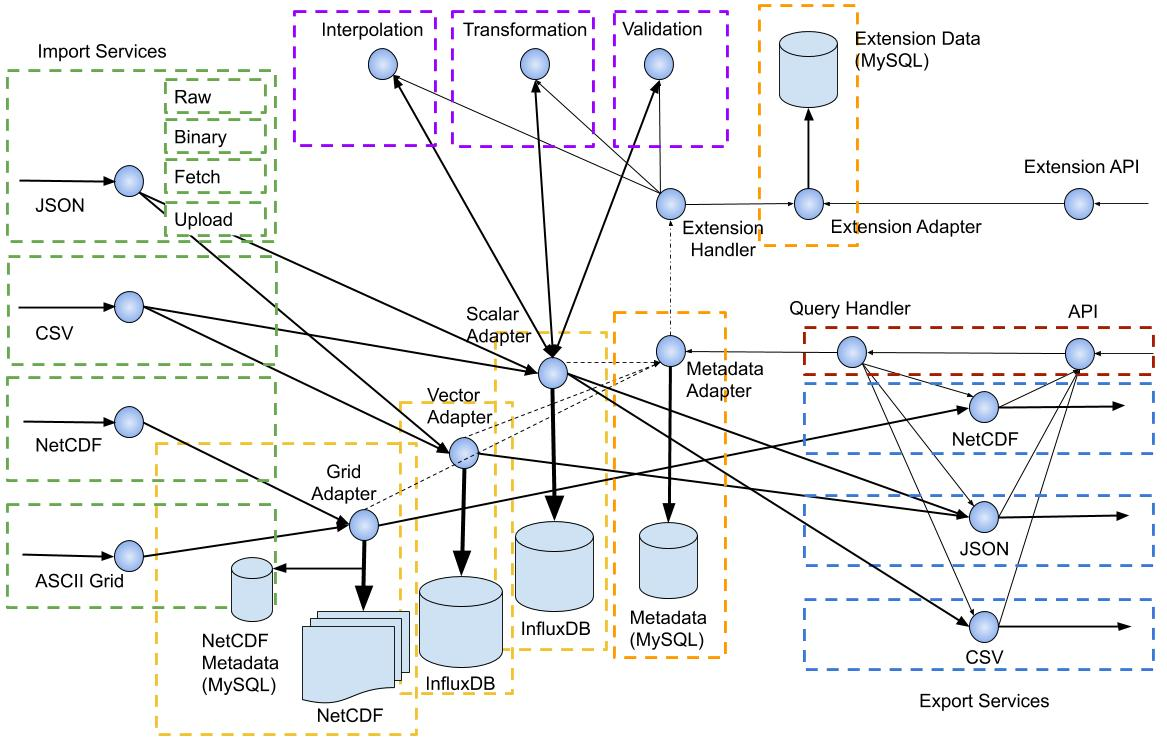
\includegraphics[width=1\textwidth]{method/microservice/separation_microservices-v3.jpg}
    \caption{Separation of \acrshort{wdias} microservices.}
    \label{fi:wdias_micro_separation}
\end{figure}
The Figure \ref{fi:wdias_micro_on_demand} show the clear separation of microservices into the modules of the \acrshort{wdias}. As it shown, each adapter has isolated database, and database is hosted separately for the high performance.
Apart from that, as we further discuss in Section \ref{se:data_preprocess}, the extension modules are running separately such as Interpolation, Transformation and Validation etc.
The Extension Adapter allow users to register new triggers for the extensions. And extension scheduler triggers the events based on time and extension handler triggers event based on data change.


%%%%%%%%%%%%%%%%%%%%%%%%%%%%%%%%%%%%%%%%%%%%%%%%%%%%%%%%%%%%%%%%%%%%%%%%%%%%%%%%
\subsection{\acrshort{wdias} API}
\label{sebse:wdias_api}
One of the main design consideration in \acrshort{wdias} is the convention of defining the APIs. It follows the simple RESTful API, and allow users to interact with HTTP methods.

\emph{Timeseries} endpoints allow to interact with Metadata Adapter, and those are cache on the Query Handler in order to perform search queries.
\begin{itemize}
    \item parameter
    \begin{itemize}
        \item \texttt{GET /parameter} -- Get parameters
        \item \texttt{POST /parameter} -- Create parameter
        \item \texttt{PUT /parameter/id} -- Update parameter
        \item \texttt{DELETE /parameter/id} -- Delete parameter
    \end{itemize}
    \item timeStep
    \begin{itemize}
        \item \texttt{GET timestep} -- Get TimeSteps
        \item \texttt{POST timestep} -- Create TimeStep
        \item \texttt{PUT timestep/id} -- Update TimeStep
        \item \texttt{DELETE timestep/id} -- Delete TimeStep
    \end{itemize}
\dbc{Format others as above}
    \item location
    \begin{itemize}
        \item \emph{GET /location} - Get location points
        \item \emph{POST /location} - Create location point
        \item \emph{PUT /location/id} - Update location point
        \item \emph{DELETE /location/id} - Delete location point
        \item \emph{GET /location/regular-grid} - Get regular grids
        \item \emph{POST /location/regular-grid} - Create regular grid
        \item \emph{PUT /location/regular-grid/id} - Update regular grid
        \item \emph{DELETE /location/regular-grid/id} - Delete regular grid
    \end{itemize}
    \item timeseries
    \begin{itemize}
        \item \emph{GET /timeseries} - Get timeseries
        \item \emph{POST /timeseries} - Create timeseries
        \item \emph{PUT /timeseries/id} - Update timeseries
        \item \emph{DELETE /timeseries/id} - Delete timeseries
    \end{itemize}
\end{itemize}

\emph{Import} endpoints allow to upload data into the \acrshort{wdias} system.
\begin{itemize}
    \item \emph{/import/json/raw}
    \item \emph{/import/ascii-grid/upload}
\end{itemize}

\emph{Export} endpoints allow to get/download data from the \acrshort{wdias} system.
\begin{itemize}
    \item \emph{/export/json/raw}
    \item \emph{/export/ascii-grid/binary}
\end{itemize}

\emph{Extensions} endpoints for configure extensions. These details describes in the Section \ref{se:data_preprocess}.

The API convention of \texttt{\hl{/MODULE/DATA\_FORMAT/DATA\_OPERATION\_TYPE}}  allows users to integrate new import or export modules into the system as well as add new data types.
